\documentclass[10pt,brazil,english]{article}
\usepackage{amsfonts}
\usepackage{infocomp}
\usepackage{times}
\usepackage{amsmath}
\usepackage{amssymb}
\usepackage[T1]{fontenc}
\usepackage[english, portuguese]{babel}
\addto\captionsportuguese{
\renewcommand{\figurename}{Figura}
\renewcommand{\tablename}{Tabela}
\renewcommand{\refname}{REFER\^{E}NCIAS}
}
\usepackage[utf8]{inputenc}
\usepackage{multirow}
\usepackage{lscape}
\usepackage{rotating}
\usepackage{setspace} % espacamento entre linhas
\usepackage[table,xcdraw]{xcolor}
\usepackage{scalefnt}
\usepackage{graphicx}
\usepackage{hyperref}
\usepackage{subfigure}
\usepackage{enumerate}
\usepackage{caption}
\usepackage[sort,compress]{cite}
\usepackage[alf,abnt-repeated-author-omit=yes,abnt-etal-list=0]{abntex2cite}	% Citações padrão ABNT
%%%%%%%%%%%%%%%%%%%%%%%%%%%%%%%%%%%%%%%%%%%%%%%%%%%%%%%%%
\usepackage{fancyhdr}
\usepackage{mathtools}
\setcounter{page}{1}
\fancyhead{ }
\lhead{}
\chead{\footnotesize SIMULAÇÃO COMPUTACIONAL DE PROCESSOS EVOLUTIVOS E SELEÇÃO NATURAL}
\rhead{}
\cfoot{}
\rfoot{\thepage}%Direita do Rodapé
\renewcommand{\headrulewidth}{1pt}% Traço horizontal no cabeçalho

%%%%%%%%%%%%%%%%%%%%%%%%%%%%%%%%%%%%%%%%%%%%%%%%%%%%%%%%%

\usepackage{rangecite}

%\hyphenation{po-pu-la-ri-za-ção re-gis-tros do-mi-na-do-ra vio-la pe-ram-bu-lam dou-tri-na-ria-men-te co-nhe-ce-rem Ad-mis-tra-ção fa-bri-car so-cie-da-de in-fe-rio-res vee-men-te-men-te si-tua-ção pon-tuais}

\sloppy
\renewcommand{\captionfont}{\footnotesize}
\renewcommand{\captionlabelfont}{\footnotesize \bfseries}
\newtheorem{exemplo}{Exemplo}
\title{SIMULAÇÃO COMPUTACIONAL DE PROCESSOS EVOLUTIVOS E SELEÇÃO NATURAL}

\address{
$^{1}$Fundação Getulio Vargas (FGV)}

\author{Lucas Emanuel Resck Domingues$^{1}$}

\selectlanguage{english}

\abstract{This assignment aims to computationally simulate biological phenomena relevant to Evolution Theory, especially with regard to natural selection. The implementation of the simulation was made in \textit{Python} through \textit{Jupyter Notebook}. Resources competitive environments were implemented, and individuals, with their own characteristics, compete there. The characteristics may favor or disfavor the adaptation of the individual to the environment. Very adapted individuals survive and reproduce, passing on their characteristics to its descendents, sometimes with mutation. The results (that are somewhat intuitive) are compared, and hypothesis are made in a try to understand them.}

\keywords{Evolution. Natural Selection. Simulation. Python. Jupyter.}

\selectlanguage{brazil}

\resumo {Este trabalho visa simular computacionalmente fenômenos biológicos pertinentes à Teoria Evolutiva, principalmente no que diz respeito à seleção natural. A implementação da simulação foi realizada na linguagem \textit{Python} através de \textit{Jupyter Notebook}. Foram implementados ambientes de competição de recursos entre indivíduos, com características próprias, que favorecem ou desfavorecerem sua adaptação ao ambiente. Indivíduos bem adaptados sobrevivem e se reproduzem, repassando essas características aos seus descendentes, às vezes com mutações. Os resultados (intuitivos, de certa forma) são comparados, e hipóteses são formuladas na tentativa de compreendê-los.}

\palchaves{Evolução. Seleção Natural. Simulação. Python. Jupyter.}

\begin{document}
    \pagestyle{fancy} % CABECALHOO
    
    \maketitle
    \newpage
    
    \section{\uppercase{Introdução}}
    
        A teoria evolutiva é uma das teorias científicas melhor consolidadas no campo da Biologia. Em geral, em quase todo problema biológico pode-se identificar uma interseção com o campo evolutivo. Dessa forma, entender a evolução e os mecanismos de seleção natural é fundamental para que quaisquer estudos e pesquisas em Biologia possam ser desenvolvidos.
        
        O presente trabalho visa demonstrar a implementação de ambientes competitivos, com recursos escassos e seleção natural, para que se verifique, através de simulações computacionais, a adaptação de indivíduos de determinada espécie, no que diz respeito às características importantes para essa adaptação. Indivíduos nascem, competem por recursos, talvez se reproduzam, assexuada ou sexuadamente, podendo gerar mutações nos seus descendentes, e, claro, morrem.
        
        Grande parte da estrutura dos ambientes implementados foi inspirada em alguns já implementados por \citeonline{Primer2018}, em sua série de vídeos exemplificando conceitos evolutivos.
        
        Esta é uma tarefa avaliada para a disciplina Modelagem de Fenômenos Biológicos, do curso de Matemática Aplicada da Fundação Getulio Vargas.
    
    \section{\uppercase{Metodologia}}
    
        A implementação dos ambientes competitivos foi realizada em \textit{Jupyter Notebook}, com a linguagem de programação \textit{Python} \cite{Lucas2019}.
        
        Foram implementados três ambientes competitivos diferentes, que são apresentados em ordem crescente de complexidade.
        
            \subsection{Ambiente com uma característica e reprodução assexuada}
            
                Vários indivíduos idênticos são iniciados ao mesmo tempo (presume-se que eles já existam), cada um deles tendo característica de velocidade (que, no início, é igual para todos). Além disso, os indivíduos possuem um grau de adaptação (\textit{fitness}), que, neste ambiente, é igual à velocidade. Sendo assim, quando mais veloz é um indivíduo, melhor adaptado ele está.
                
                O ambiente possui recursos de comida limitados. A distribuição dessas comidas em um período de tempo chamado dia é feita uma a uma (em rodadas), até que todas as comidas sejam distribuídas ou não haja mais indivíduos capazes de recebê-las neste dia. Além disso, a distribuição aos indivíduos ocorre de acordo com probabilidades proporcionais aos graus de adaptação dos indivíduos. Portanto, indivíduos melhor adaptados têm maiores probabilidades de conseguir comida.
                
                Indivíduos têm energia, e cada rodada de distribuição que um indivíduo participa consome uma parte dessa energia, parte esta influenciada pela característica de velocidade. Neste ambiente, a cada rodada de distribuição, os indivíduos que estiverem buscando por comida têm subtraídos de sua energia o valor de sua velocidade ao quadrado. Sendo assim, é possível que, em um determinado dia, um indivíduo não participe de todas as rodadas de distribuição de comida.
                
                Se um indivíduo consegue uma comida, ele sobrevive para o próximo dia. Se ele consegue duas comidas, ele sobrevive para o próximo dia e se reproduz assexuadamente: quem nasce é um clone, porém com uma probabilidade de mutação na característica da velocidade. Aqueles indivíduos que não conseguem nenhuma comida até o fim da distribuição no dia morrem (não participam mais da simulação).
                
                Ao fim do dia, as energias são reestabelecidas e as comidas acabam, e o processo reinicia. Isso ocorre durante vários dias.
                
                Durante a implementação, podem ser escolhidas algumas características do processo: velocidade inicial, quantidade inicial de comida, energia inicial, probabilidade de mutação e número de dias.
                
                Os ambientes foram testados com alguns parâmetros diferentes para verificar como a população de indivíduos se comporta diante desses parâmetros.
            
            \subsection{Ambiente com várias características, morte por idade e reprodução assexuada}
            
                Este ambiente tem algumas poucas diferenças em relação ao anterior. Além da característica de velocidade, os indivíduos possuem peso e tamanho. Agora, o grau de adaptação é o resultado da soma dessas três características. Durante a reprodução (assexuada), cada um desses fatores pode sofrer mutação, independentemente dos outros.
                
                Em cada rodada de distribuição de comida, os indivíduos que participam têm descontados de sua energia o valor de sua velocidade ao quadrado, o valor de seu tamanho ao cubo e o valor do seu peso. O motivo pelo qual escolhi, por exemplo, subtrair o tamanho ao cubo, e não apenas o tamanho, foi tentar representar, de forma intuitiva, como o tamanho consome energia em um ser, pois a energia está relacionada não ao tamanho, mas ao seu volume, de certa forma. Essa ideia intuitiva foi explorada por \citeonline{Primer2018}.
                
                Além disso, os seres morrem por idade, sendo esta idade determinada antes da simulação.
            
            \subsection{Ambiente com várias características, morte por idade e reprodução sexuada}
            
                Este ambiente é análogo ao anterior, modificado apenas para incluir a reprodução sexuada. Os indivíduos têm sexo, determinado aleatoriamente no início de sua vida.
                
                Aqueles seres que recebem duas comidas durante um dia são aqueles com a capacidade de se reproduzir durante esse dia.
                
                Entre os indivíduos capazes de se reproduzir, os seres melhor adaptados de um sexo se reproduzem com os melhor adaptados do outro. Como o número de seres capazes de se reproduzir em um determinado dia pode ser diferente entre os sexos, pode haver indivíduos que não se reproduzem, mas são capazes disso, nesse dia.
                
                O indivíduo resultado do cruzamento de dois seres tem suas características iguais às médias aritméticas das características dos seus pais, com uma probabilidade de mutação em cada fator: velocidade, tamanho e peso.
    
    \section{\uppercase{Resultados e Discussões}}
    
        \subsection{Ambiente com uma característica e reprodução assexuada}
        
            A Tabela \ref{Tab1} mostra os parâmetros utilizados na primeira simulação:
            
            \begin{table}[!hbtp]
                \centering
                \caption{Parâmetros utilizados na primeira simulação no primeiro ambiente.}
                \label{Tab1}
                \begin{tabular}{c|c}
                    \hline
                    \textbf{Parâmetro}          & \textbf{Valor}    \\ \hline
                    Número de indivíduos        & 100               \\ \hline
                    Velocidade inicial          & 2                 \\ \hline
                    Energia                     & 100               \\ \hline
                    Probabilidade de mutação    & 0,5\%             \\ \hline
                    Número de dias              & 1000              \\ \hline
                    Comidas disponíveis         & 50                \\ \hline
                \end{tabular}
            \end{table}
            
            Como cada indivíduo, durante um dia, tem seu próprio grau de adaptação, na Figura \ref{Fig1} é mostrada a média dos graus de adaptação no tempo (em dias). As Figuras \ref{Fig2} e \ref{Fig3} apresentam o desvio padrão dos graus de adaptação e o número de indivíduos, no tempo.
            
            \begin{figure}[!hbtp]
                \begin{center}
                    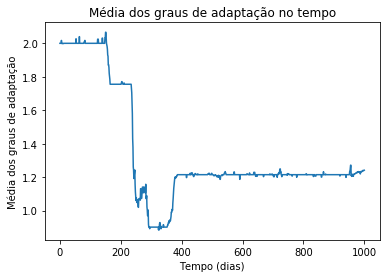
\includegraphics[scale=0.5]{Images/1-1.png}
                \end{center}
                \caption{Média dos graus de adaptação no tempo na primeira simulação no primeiro ambiente.}
                \label{Fig1}
            \end{figure} 
            
            \begin{figure}[!hbtp]
                \begin{center}
                    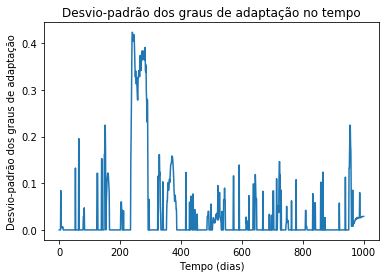
\includegraphics[scale=0.5]{Images/1-2.png}
                \end{center}
                \caption{Desvio-padrão dos graus de adaptação no tempo na primeira simulação no primeiro ambiente.}
                \label{Fig2}
            \end{figure} 
            
            \begin{figure}[!hbtp]
                \begin{center}
                    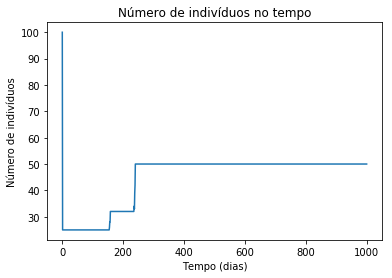
\includegraphics[scale=0.5]{Images/1-3.png}
                \end{center}
                \caption{Número de indivíduos no tempo na primeira simulação no primeiro ambiente.}
                \label{Fig3}
            \end{figure}
            
            Observamos que a média dos graus de adaptação tende a se estabelecer em 1,2, com baixo desvio-padrão. Além disso, o número de indivíduos se mantém constante em 50 a partir de certo dia.
            
            A Tabela \ref{Tab2} mostra os parâmetros utilizados para a segunda simulação. Veja que a velocidade inicial de cada indivíduo é bem menor do que na primeira.
            
            \begin{table}[!hbtp]
                \centering
                \caption{Parâmetros utilizados na segunda simulação no primeiro ambiente.}
                \label{Tab2}
                \begin{tabular}{c|c}
                    \hline
                    \textbf{Parâmetro}          & \textbf{Valor}    \\ \hline
                    Número de indivíduos        & 100               \\ \hline
                    Velocidade inicial          & 0,5               \\ \hline
                    Energia                     & 100               \\ \hline
                    Probabilidade de mutação    & 0,5\%             \\ \hline
                    Número de dias              & 1000              \\ \hline
                    Comidas disponíveis         & 50                \\ \hline
                \end{tabular}
            \end{table}
            
            As Figuras \ref{Fig4}, \ref{Fig5} e \ref{Fig6} mostram, respectivamente, gráficos da média dos graus de adaptação, do desvio-padrão dos graus de adaptação e do número de indivíduos, no tempo, para essa simulação:
            
            \begin{figure}[!hbtp]
                \begin{center}
                    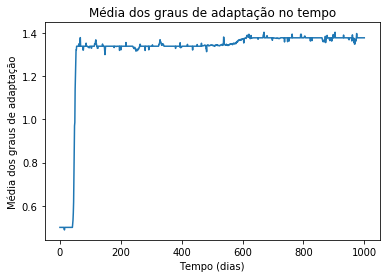
\includegraphics[scale=0.5]{Images/1-4.png}
                \end{center}
                \caption{Resultados da média dos graus de adaptação no tempo na segunda simulação no primeiro ambiente.}
                \label{Fig4}
            \end{figure} 
            
            \begin{figure}[!hbtp]
                \begin{center}
                    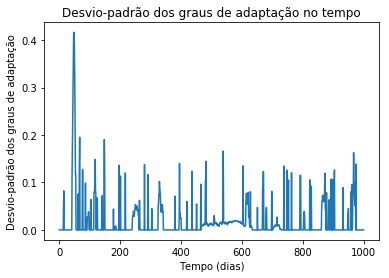
\includegraphics[scale=0.5]{Images/1-5.png}
                \end{center}
                \caption{Resultados do desvio-padrão dos graus de adaptação no tempo na segunda simulação no primeiro ambiente.}
                \label{Fig5}
            \end{figure} 
            
            \begin{figure}[!hbtp]
                \begin{center}
                    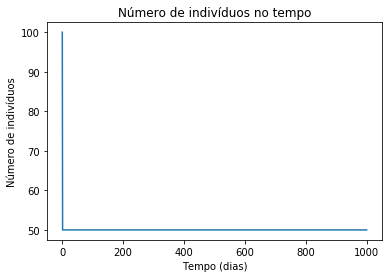
\includegraphics[scale=0.5]{Images/1-6.png}
                \end{center}
                \caption{Resultados do número de indivíduos no tempo na segunda simulação no primeiro ambiente.}
                \label{Fig6}
            \end{figure}
            
            Nesta segunda simulação, podemos notar que a média dos graus de adaptação também tende a um valor, neste caso 1,4, próximo ao da simulação anterior. Além disso, o número de indivíduos também se mantém em 50.
            
            É curioso que o número de indivíduos nas duas simulações se manteve constante a partir de certo momento, inclusive no mesmo valor: 50. A explicação é direta: há 50 comidas, portanto há comida para no máximo 50 indivíduos. Se um indivíduo fica sem comida, algum outro terá essa comida, ficando com duas e, portanto, se reproduzindo. Isso mantém o número de seres constante em 50.
            
            Durante algumas simulações, às vezes, esse número não é constante, caindo para 49, por exemplo. Isso ocorre porque existe uma possibilidade de que tenhamos 50 indivíduos vivos apenas, e o indivíduo que receberia a 50ª comida não tenha energia para participar da última rodada. Ele morre, diminuindo a população para 49.
            
            Observe como nos dois ambientes a média dos graus de adaptação convergiu para valores, que inclusive são próximos. Esse valor, que supomos ser ótimo, ou pelo menos próximo do ótimo, aparentemente não depende das características iniciais dos indivíduos.
            
            Qual seria uma hipótese razoável de por que houve uma convergência para um valor de velocidade entre 1,2 e 1,4 nesse ambiente?  Considerando que o número de rodadas de distribuição de comida é 50 e a energia dos indivíduos é 100, para que ele participe de todas as rodadas de distribuição o desconto em cada rodada precisa ser igual a 2.  Como o desconto é o quadrado da velocidade, basta que a velocidade seja aproximadamente 1,4. Esse valor, portanto, garante que todos os 50 indivíduos participem de  todas  as  rodadas,  com  grau  de adaptação  máximo seguindo esse critério.
            
            Não só a média dos graus de adaptação aparenta convergir para alguns valores nas duas simulações, como há uma tendência de diminuição do desvio-padrão dos graus de adaptação, mesmo ele sendo pequeno. Ou seja, os próprios graus de adaptação estão mais próximos da média.
            
        \subsection{Ambiente com várias características, morte por idade e reprodução assexuada}
        
            A Tabela \ref{Tab3} apresenta os parâmetros desta simulação.
            
            \begin{table}[!hbtp]
                \centering
                \caption{Parâmetros utilizados na primeira simulação no segundo ambiente.}
                \label{Tab3}
                \begin{tabular}{c|c}
                    \hline
                    \textbf{Parâmetro}          & \textbf{Valor}    \\ \hline
                    Número de indivíduos        & 100               \\ \hline
                    Velocidade inicial          & 2                 \\ \hline
                    Tamanho inicial             & 2                 \\ \hline
                    Peso inicial                & 2                 \\ \hline
                    Energia                     & 100               \\ \hline
                    Probabilidade de mutação    & 0,5\%             \\ \hline
                    Idade de morte (dias)       & 10                \\ \hline
                    Número de dias              & 5000              \\ \hline
                    Comidas disponíveis         & 50                \\ \hline
                \end{tabular}
            \end{table}
            
            As Figuras \ref{Fig7}, \ref{Fig8} e \ref{Fig9} apresentam a média das caracerísticas (velocidade, tamanho e peso) e do grau de adaptação, o desvio-padrão desses fatores e o número de indivíduos, respectivamente, variando no tempo, em dias.
            
            \begin{figure}[!hbtp]
                \begin{center}
                    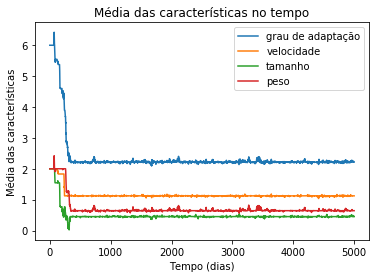
\includegraphics[scale=0.5]{Images/2-1.png}
                \end{center}
                \caption{Resultados da média das características no tempo na primeira simulação no segundo ambiente.}
                \label{Fig7}
            \end{figure} 
            
            \begin{figure}[!hbtp]
                \begin{center}
                    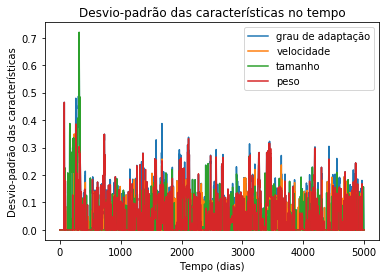
\includegraphics[scale=0.5]{Images/2-2.png}
                \end{center}
                \caption{Resultados do desvio-padrão das características no tempo na primeira simulação no segundo ambiente.}
                \label{Fig8}
            \end{figure} 
            
            \begin{figure}[!hbtp]
                \begin{center}
                    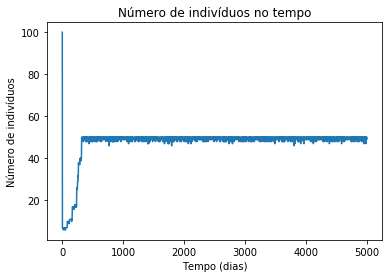
\includegraphics[scale=0.5]{Images/2-3.png}
                \end{center}
                \caption{Resultados do número de indivíduos no tempo na primeira simulação no segundo ambiente.}
                \label{Fig9}
            \end{figure}
            
            Logo no início da simulação, todas as características, e consequentemente o grau de adaptação, tendem a um valor. Com baixos desvios-padrões, a velocidade se mantém pŕoxima de 1,1, o tamanho se mantém em torno de 0,5 e o peso, por sua vez, 0,6. Sendo assim, o grau de adaptação tende a ficar próximo de 2,2. O número de indivíduos também fica próximo de 50, porém não é mais constante, como nas simulações anteriores.
            
            Para a segunda simulação neste ambiente, a Tabela \ref{Tab4} apresenta os parâmetros escolhidos.
            
            \begin{table}[!hbtp]
                \centering
                \caption{Parâmetros utilizados na segunda simulação no segundo ambiente.}
                \label{Tab4}
                \begin{tabular}{c|c}
                    \hline
                    \textbf{Parâmetro}          & \textbf{Valor}    \\ \hline
                    Número de indivíduos        & 100               \\ \hline
                    Velocidade inicial          & 0,1               \\ \hline
                    Tamanho inicial             & 0,1               \\ \hline
                    Peso inicial                & 0,1               \\ \hline
                    Energia                     & 100               \\ \hline
                    Probabilidade de mutação    & 0,5\%             \\ \hline
                    Idade de morte (dias)       & 10                \\ \hline
                    Número de dias              & 5000              \\ \hline
                    Comidas disponíveis         & 50                \\ \hline
                \end{tabular}
            \end{table}
            
            As Figuras \ref{Fig10}, \ref{Fig11} e \ref{Fig12} mostram gráficos, respectivamente, da média das características (e grau de adaptação), do desvio-padrão desses fatores e do número de indivíduos, todos no tempo.
            
            \begin{figure}[!hbtp]
                \begin{center}
                    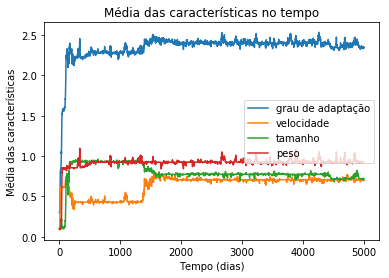
\includegraphics[scale=0.5]{Images/2-4.png}
                \end{center}
                \caption{Resultados da média das características no tempo na segunda simulação no segundo ambiente.}
                \label{Fig10}
            \end{figure} 
            
            \begin{figure}[!hbtp]
                \begin{center}
                    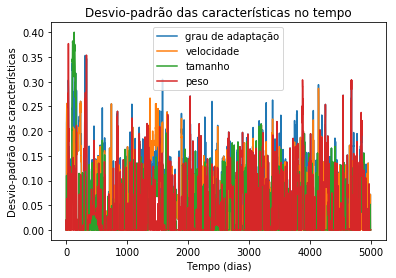
\includegraphics[scale=0.5]{Images/2-5.png}
                \end{center}
                \caption{Resultados do desvio-padrão das características no tempo na segunda simulação no segundo ambiente.}
                \label{Fig11}
            \end{figure} 
            
            \begin{figure}[!hbtp]
                \begin{center}
                    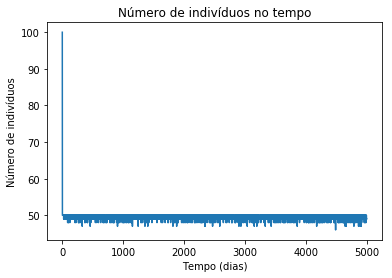
\includegraphics[scale=0.5]{Images/2-6.png}
                \end{center}
                \caption{Resultados do número de indivíduos no tempo na segunda simulação no segundo ambiente.}
                \label{Fig12}
            \end{figure}
            
            Com desvios-padrões um pouco mais altos, a velocidade e o tamanho procuram se manter perto de 0,7, e o peso, 0,9. Portanto, o grau de adaptação se mantém em torno de 2,3. Observe que, como na simulação na anterior, o número de indivíduos se mantém próximo de 50, porém não constante. Provavelmente isso ocorre porque os indivíduos morrem depois de 10 dias vivos.
            
            Nas duas simulações neste ambiente, os valores para os quais as médias dos graus de adaptação convergem são próximos entre si. É uma evidência de que estão próximos de um valor ótimo, ou um valor próximo do ótimo. É curioso notar, porém, que os valores para os quais as médias das características (e não a soma delas) convergem são diferentes nas duas simulações. Por exemplo, na Figura \ref{Fig7}, a velocidade fica em torno de 1,1, enquanto, na Figura \ref{Fig10}, ela fica próxima de 0,7. Ou seja, pode existir mais de uma configuração ideal para as características na população.
            
            É possível notar, também neste ambiente, uma pequena tendência de diminuição dos desvios-padrões, sendo que eles também são pequenos. Ou seja, os próprios valores das características convergindo para a média.
        
        \subsection{Ambiente com várias características, morte por idade e reprodução sexuada}
        
            A Tabela \ref{Tab5} apresenta os parâmetros escolhidos para essa simulação.
            
            \begin{table}[!hbtp]
                \centering
                \caption{Parâmetros utilizados na primeira simulação no terceiro ambiente.}
                \label{Tab5}
                \begin{tabular}{c|c}
                    \hline
                    \textbf{Parâmetro}          & \textbf{Valor}    \\ \hline
                    Número de indivíduos        & 100               \\ \hline
                    Velocidade inicial          & 1,2               \\ \hline
                    Tamanho inicial             & 1,2               \\ \hline
                    Peso inicial                & 1,2               \\ \hline
                    Energia                     & 100               \\ \hline
                    Probabilidade de mutação    & 0,5\%             \\ \hline
                    Idade de morte (dias)       & 10                \\ \hline
                    Número de dias              & 5000              \\ \hline
                    Comidas disponíveis         & 50                \\ \hline
                \end{tabular}
            \end{table}
            
            As Figuras \ref{Fig13}, \ref{Fig14} e \ref{Fig15} apresentam a média das caracerísticas (velocidade, tamanho e peso) e do grau de adaptação, o desvio-padrão desses fatores e o número de indivíduos, respectivamente, todos no tempo, medido em dias.
            
            \begin{figure}[!hbtp]
                \begin{center}
                    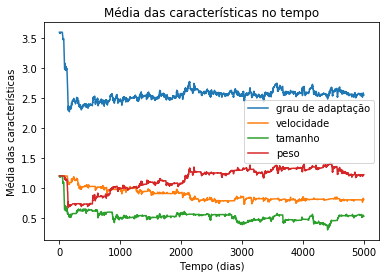
\includegraphics[scale=0.5]{Images/3-1.png}
                \end{center}
                \caption{Resultados da média das características no tempo na primeira simulação no terceiro ambiente.}
                \label{Fig13}
            \end{figure} 
            
            \begin{figure}[!hbtp]
                \begin{center}
                    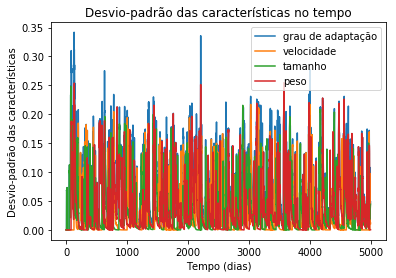
\includegraphics[scale=0.5]{Images/3-2.png}
                \end{center}
                \caption{Resultados do desvio-padrão das características no tempo na primeira simulação no terceiro ambiente.}
                \label{Fig14}
            \end{figure} 
            
            \begin{figure}[!hbtp]
                \begin{center}
                    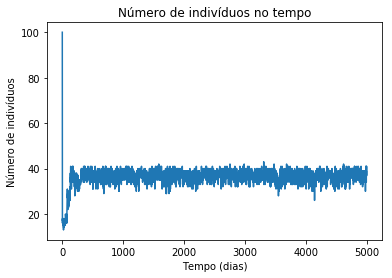
\includegraphics[scale=0.5]{Images/3-3.png}
                \end{center}
                \caption{Resultados do número de indivíduos no tempo na primeira simulação no terceiro ambiente.}
                \label{Fig15}
            \end{figure}
            
            Observamos que as características tendem a se tornar um pouco menos constantes. A velocidade se mantém perto de 0,8, tamanho se mantém em torno de 0,5 e peso, por sua vez, 1,2. Sendo assim, o grau de adaptação tende a ficar próximo de 2,6. O número de indivíduos fica próximo de 40, de forma não constante.
            
            Os parâmetros para a segunda simulação neste ambiente se encontram na Tabela \ref{Tab6}.
            
            \begin{table}[!hbtp]
                \centering
                \caption{Parâmetros utilizados na primeira simulação no terceiro ambiente.}
                \label{Tab6}
                \begin{tabular}{c|c}
                    \hline
                    \textbf{Parâmetro}          & \textbf{Valor}    \\ \hline
                    Número de indivíduos        & 100               \\ \hline
                    Velocidade inicial          & 0,1               \\ \hline
                    Tamanho inicial             & 0,1               \\ \hline
                    Peso inicial                & 0,1               \\ \hline
                    Energia                     & 100               \\ \hline
                    Probabilidade de mutação    & 0,5\%             \\ \hline
                    Idade de morte (dias)       & 10                \\ \hline
                    Número de dias              & 5000              \\ \hline
                    Comidas disponíveis         & 50                \\ \hline
                \end{tabular}
            \end{table}
            
            As Figuras \ref{Fig16}, \ref{Fig17} e \ref{Fig18} mostram gráficos da média das características e do grau de adaptação, do desvio-padrão desses fatores e do número de indivíduos, respectivamente.
            
            \begin{figure}[!hbtp]
                \begin{center}
                    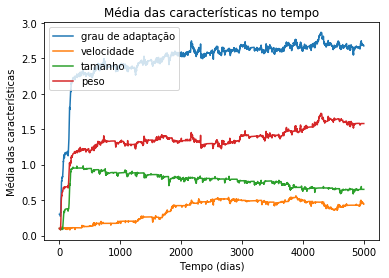
\includegraphics[scale=0.5]{Images/3-4.png}
                \end{center}
                \caption{Resultados da média das características no tempo na segunda simulação no terceiro ambiente.}
                \label{Fig16}
            \end{figure} 
            
            \begin{figure}[!hbtp]
                \begin{center}
                    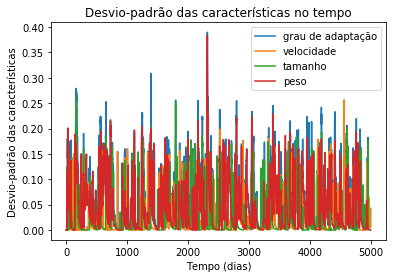
\includegraphics[scale=0.5]{Images/3-5.png}
                \end{center}
                \caption{Resultados do desvio-padrão das características no tempo na segunda simulação no terceiro ambiente.}
                \label{Fig17}
            \end{figure} 
            
            \begin{figure}[!hbtp]
                \begin{center}
                    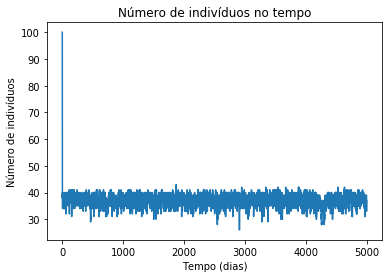
\includegraphics[scale=0.5]{Images/3-6.png}
                \end{center}
                \caption{Resultados do número de indivíduos no tempo na segunda simulação no terceiro ambiente.}
                \label{Fig18}
            \end{figure}
            
            Aqui, as características se tornaram menos constantes ainda, em comparação com as outras simulações presentes neste trabalho. A velocidade se mantém em torno de 0,4, o tamanho, 0,65, e o peso, 1,6, resultando em um grau de adaptação perto de 2,7. A população também não é constante, em torno de 40 indivíduos.
            
            Nesse ambiente, os resultados tiveram duas diferenças principais, se comparados aos outros: a não constância das características e a mudança de valor em torno do qual fica o número de indivíduos.
            
            À medida que o modelo fica mais complexo, é de se esperar que o modelo fique menos previsível, ou seja, as características fiquem menos constantes. Além disso, no que diz respeito ao número de indivíduos, é interessante notar que, agora, nem todos os indivíduos capazes de se reproduzir (aqueles com duas comidas) se reproduzem, pois o número de seres capazes pode diferir entre os sexos. Por exemplo, podem sobrar machos capazes. Assim, aquela comida que teria como destino a reprodução (e que algum outro ser morreu por não tê-la recebido) não cumpre esse objetivo, diminuindo a população.
    
    \section{\uppercase{Considerações Finais}} 
    
        Em todas as simulações em todos os ambientes, a média dos graus de adaptação tende a um valor que aparenta ser ótimo, ou pelo menos muito bom. Mais do que isso: em um mesmo ambiente, em simulações com parâmetros parecidos, porém com características iniciais diferentes, a média dos graus de adaptação tende a valores próximos. Ou seja, esse valor ótimo, ou pelo menos muito bom, não depende das características iniciais da simulação.
        
        Vamos considerar o primeiro ambiente (com característica de velocidade apenas). Nas duas simulações, a média dos graus de adaptação tendem a algo entre 1,2 e 1,4, como podemos verificar nas Figuras \ref{Fig1} e \ref{Fig4}, respectivamente. Na primeira simulação, o valor inicial de velocidade é 2, e, na segunda, 0,5. Esse valor ótimo, ou pelo menos muito bom, pode ser interpretado como o valor de velocidade que maximiza o grau de adaptação em conjunto com o número de rodadas de distribuição que o indivíduo vai participar.
        
        Podemos pensar: uma velocidade baixa, no primeiro ambiente, significa baixo grau de adaptação, porém muitas rodadas de distribuição, pois se consome pouca energia; alta velocidade, por sua vez, significa alto grau de adaptação, e um número menor de rodadas.
        
        Em todas as simulações, principalmente nas iniciais, é possível ver uma tendência de diminuição do desvio-padrão das características no tempo, mesmo que sej uma pequena inclinação e que o próprio desvio-padrão seja pequeno.
    
        Foram apresentados três modelos, ordenados por complexidade, de maneira crescente. O primeiro modelo, muito simples, após a convergência da média dos graus de adaptação, tende a manter esse valor durante o tempo, sem oscilações (veja a Figura \ref{Fig1}). Já no último modelo, essa convergência não é tão fácil de ser reconhecida, e a média dos graus de adaptação oscila em torno de um valor não trivial de ser estimado (veja a Figura \ref{Fig16}). Isso é esperado, pois, intuitivamente, tendemos a considerar que a convergência está relacionada à simplicidade.
        
        Na verdade, a maioria dos, se não todos os, resultados apresentados são intuitivos, e demonstram o caráter algorítmico da seleção natural: indivíduos são diferentes devido aos cruzamentos e às mutações, e aqueles melhor adaptados são selecionados para perpertuar suas características, inclusive as próprias características que os tornam melhor adaptados.
    
    \bibliography{Referencias}
    
    \nocite{carykh2015}

\end{document} 